\documentstyle[11pt,epsfig,fancybox,semcolor,semlayer,doublespace,portrait]
{seminar}
\input clp_utils

\def\ys{$\Upsilon(1S)$}
\def\yss{$\Upsilon(2S)$}
\def\ysss{$\Upsilon(3S)$}
\def\gamee{$\Gamma_{e^+e^-}$}

% The following strings are needed by the title page and 
% page style definitions in map_utils.tex
\newcommand{\talktitle}[0]{\gamee for \ys, \yss\  and \ysss}
\newcommand{\fmttitle}[0]{}
\newcommand{\conftitle}[0]{September 2002 CLEO Meeting}
\newcommand{\myname}[0]{Jim Pivarski}
\newcommand{\affila}[0]{Cornell University}
\newcommand{\talkdate}[0]{September 13, 2002}

\pagestyle{conference}   % From clp_utils.tex

% slide magnification
\slidesmag 1

%%%%%%%%%%%%%%%%%%%%%%%%%%%%%%%%%%%%%%%%%%%%%%%%%%%%%%%%%%%%%%%%%%%%%%%%%%%
% Start document
\begin{document}

% Set page size
\slideheight 7.0in
\slidewidth 8.8in 

% Set array stretch
\renewcommand{\arraystretch}{0.3}
\renewcommand{\slidetopmargin}{0.4in}
\renewcommand{\slidebottommargin}{0.9in}


%%%%%%%%%%%%%%%%%%%%%%%%%%%%%%%%%%%%%%%%%%%%%%%%%%%%%%%%%%%%%%%%%%%%%%%%%%%

\begin{slide*}

\slideframe{}
\slideframe*[\dkblue]{Oval}

\begin{center}
\vspace{4 cm}
{\Huge \black Generic (Pass2!) Cuts for Upsilon Scans } \\
{\LARGE \black	Jim Pivarski } \\
% \vspace{0.25 cm}
% {\LARGE	Ritchie Patterson } \\
% \vspace{0.25 cm}
% {\LARGE	Karl Berkelman } \\
\vspace{2 cm}
\conftitle \\
{\large \black \talkdate}

\end{center}

\end{slide*}

% %%%%%%%%%%%%%%%%%%%%%%%%%%%%%%%%%%%%%%%%%%%%%%%%%%%%%%%%%%%%%%%%%%%%%%%%%%%

% \begin{slide*}

% \slideframe{}
% \slideframe*[\dkblue]{Oval}
% \huge
% \heading{Outline}
% \vspace{1 cm}

% \begin{center}
% \begin{minipage}[t]{12 cm}
% \begin{itemize}
% \LARGE \item {\huge Motivation: verify lattice QCD!}
% \LARGE \item {\huge 2 out of 3 Resonances Scanned}
% \LARGE \item {\huge Energy Calibration Systematics}
% \LARGE \item {\huge Other Systematics / Work to be Done}
% \end{itemize}
% \end{minipage}
% \end{center}

% \end{slide*}
 
%%%%%%%%%%%%%%%%%%%%%%%%%%%%%%%%%%%%%%%%%%%%%%%%%%%%%%%%%%%%%%%%%%%%%%%%%%%

\begin{slide*}

\slideframe{}
\slideframe*[\dkblue]{Oval}
\huge
\heading{Last time\ldots}

\begin{minipage}[t]{\linewidth}
\LARGE

\begin{itemize}
  \item Datataking on the \yss\ was starting. Now it's finished.

  \item I decided that ``Weighted Average$\large\{$track $z_0\large\}$''
  was a good variable to cut out beam gas/wall/cosmic rays (cut at 10 cm).

\begin{center}
  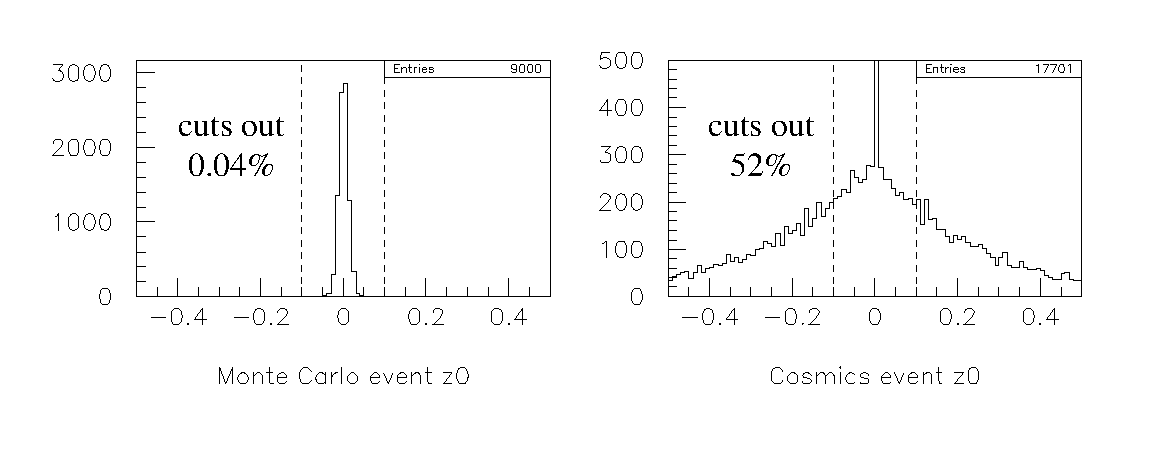
\epsfig{file=talk_wz0_2.eps,width=\linewidth} \\
\end{center}

  \item But I was looking for a good cut in 2D\ldots

\end{itemize}

\end{minipage}

\end{slide*}

%%%%%%%%%%%%%%%%%%%%%%%%%%%%%%%%%%%%%%%%%%%%%%%%%%%%%%%%%%%%%%%%%%%%%%%%%%%

\begin{slide*}

\slideframe{}
\slideframe*[\dkblue]{Oval}
\huge
\heading{2D Cut: Closest Intersection}

\begin{minipage}[t]{\linewidth}
\LARGE

I found one! Here's the algorithm:

\begin{enumerate}
  \item In the 2D projection, find all intersections of pairs of tracks.

\begin{center}
  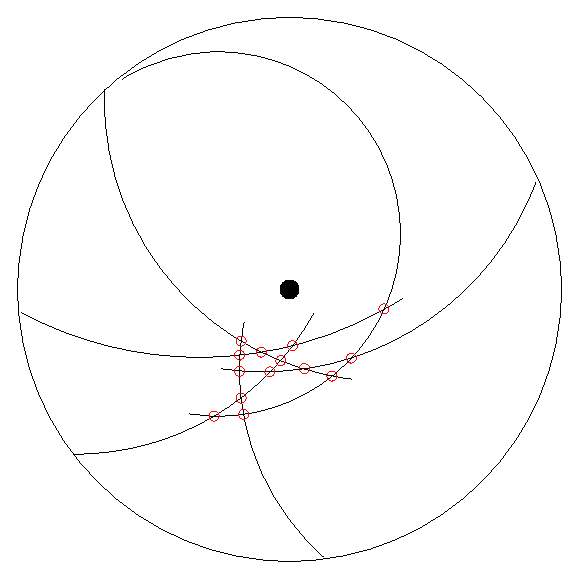
\epsfig{file=crossings_2d.eps,width=0.5\linewidth} \\
\end{center}

  \item Pick the one which is closest to the beamspot.

  \item Cut on the distance to this ``closest intersection'' at 3 mm.

\end{enumerate}

\end{minipage}

\end{slide*}

%%%%%%%%%%%%%%%%%%%%%%%%%%%%%%%%%%%%%%%%%%%%%%%%%%%%%%%%%%%%%%%%%%%%%%%%%%%

\begin{slide*}

\slideframe{}
\slideframe*[\dkblue]{Oval}
\huge
\heading{2D Cut: Closest Intersection}

\begin{minipage}[t]{\linewidth}
\LARGE

\vspace{1 in}

\begin{center}
  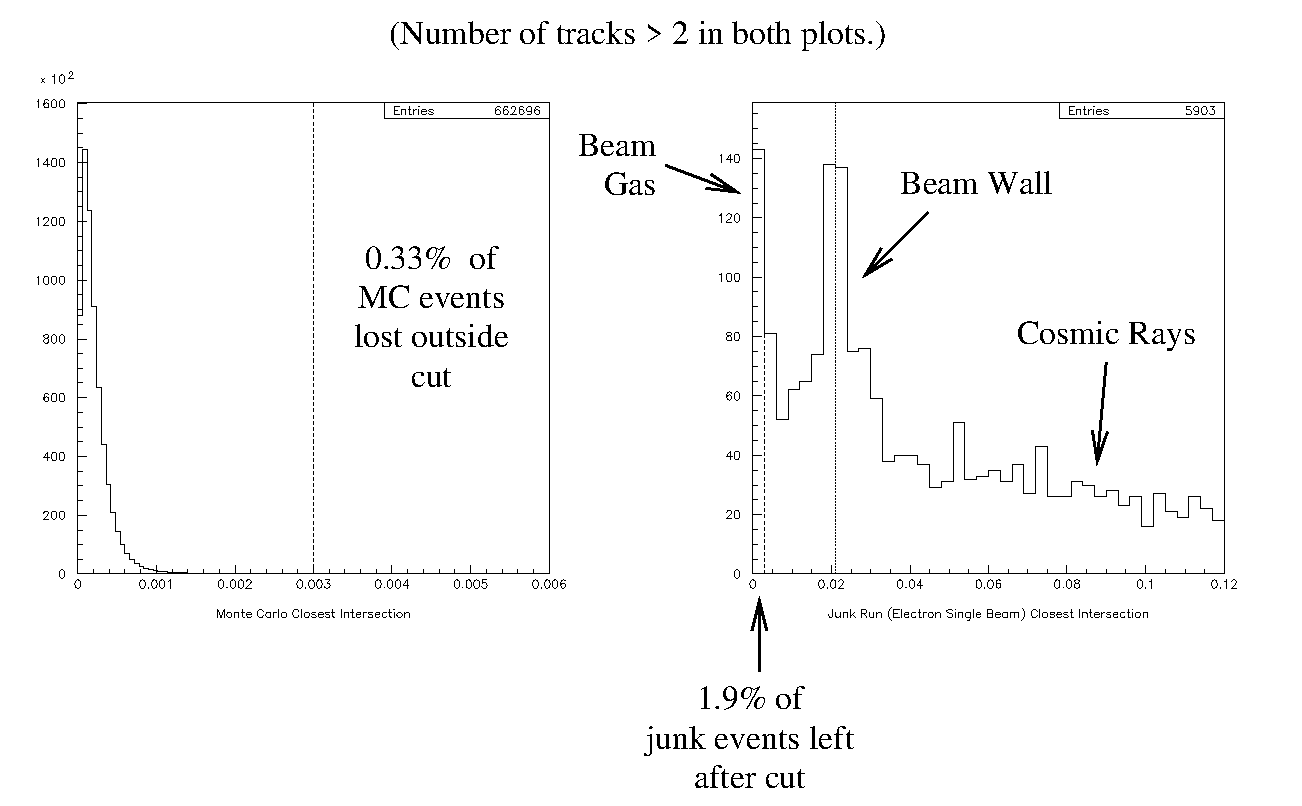
\epsfig{file=closest_intersection.eps,width=\linewidth} \\
\end{center}

\end{minipage}

\end{slide*}

%%%%%%%%%%%%%%%%%%%%%%%%%%%%%%%%%%%%%%%%%%%%%%%%%%%%%%%%%%%%%%%%%%%%%%%%%%%

\begin{slide*}

\slideframe{}
\slideframe*[\dkblue]{Oval}
\huge
\heading{Generic Set of Cuts}

\begin{minipage}[t]{\linewidth}
\LARGE

\begin{itemize}
  \item Loose Geometrical cuts

\begin{center}
  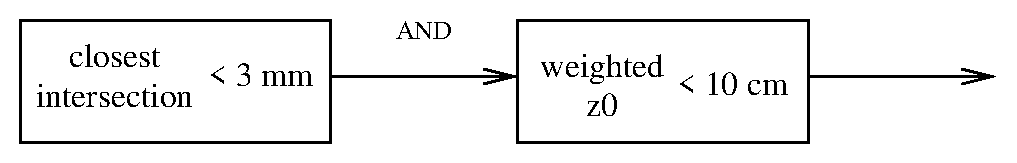
\epsfig{file=geometrica.eps, width=0.5\linewidth} \\
\end{center}

  \item ``Hadron Subcollection'' cuts

\begin{center}
  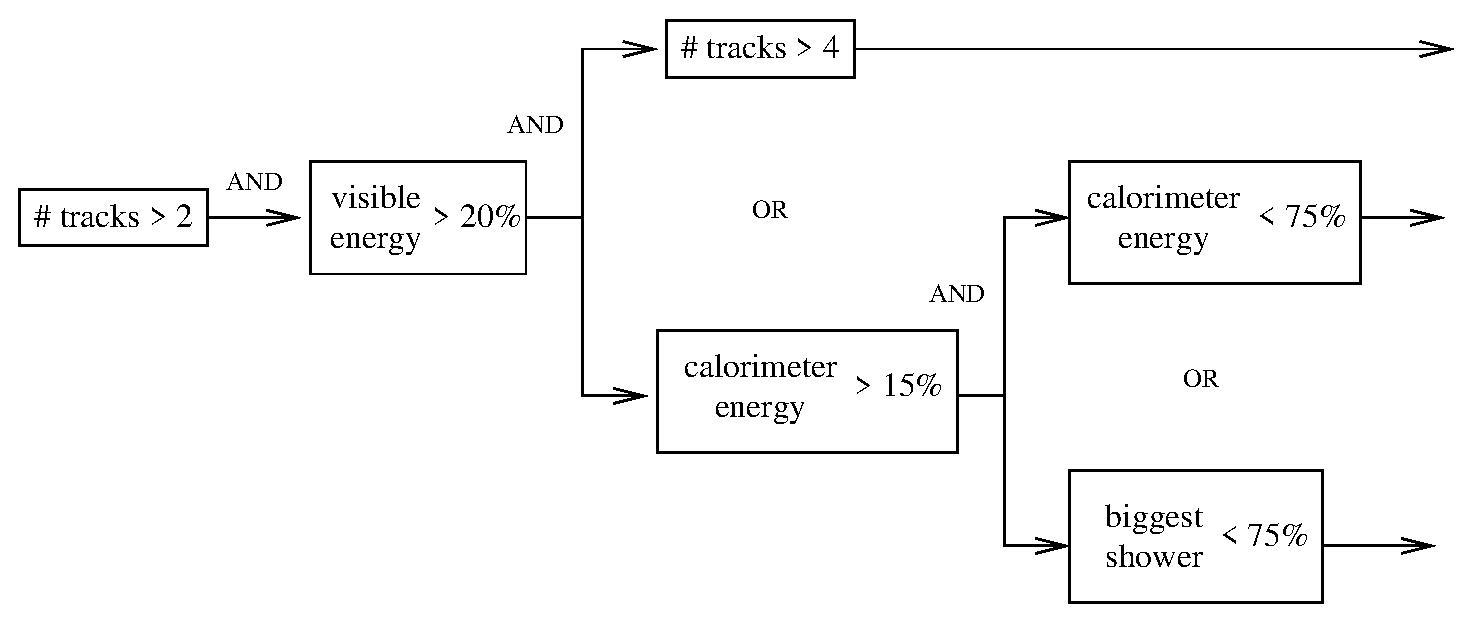
\epsfig{file=hadron.eps, width=0.8\linewidth} \\
\end{center}

  \item Possibly more, to supress specific backgrounds.

\end{itemize}

\vspace{0.5 in}

(Calorimeter energy cut reduces cosmic ray contribution in single beam
data by an additional 4\%.)

\end{minipage}

\end{slide*}

%%%%%%%%%%%%%%%%%%%%%%%%%%%%%%%%%%%%%%%%%%%%%%%%%%%%%%%%%%%%%%%%%%%%%%%%%%%

\begin{slide*}

\slideframe{}
\slideframe*[\dkblue]{Oval}
\huge
\heading{Background Studies}

\begin{minipage}[t]{\linewidth}
\large

{\LARGE Now I can begin to look seriously at backgrounds.}

\vspace{1 cm}

\begin{tabular}{l c c c}
Background & Contribution to Data$^1$ & Scaling & Bias at Peak \\\hline
Continuum hadron & 73.9\% & $1/s$ & 0 \\
Bhabha & 0.15\% & $1/s$ & 0 \\
Tau & 5.1\% & $1/s$ & 0 \\
Cosmic Rays & $<$ 0.04\%$^2$ & with time & $<$ 0.04\% \\
Beam Gas & 1\% & with current$^2$ & 0.15\% \\
Two-Photon$^3$ & 19\% & $\log s$ & 0.026\% \\
\end{tabular}

\vspace{1 cm}

$^1$ At the continuum energy point.

$^2$ A more complete cosmic ray study is planned.

$^3$ The two-photon contribution is currently normalized by
subtracting the other sources.

\end{minipage}

\end{slide*}

%%%%%%%%%%%%%%%%%%%%%%%%%%%%%%%%%%%%%%%%%%%%%%%%%%%%%%%%%%%%%%%%%%%%%%%%%%%

\begin{slide*}

\slideframe{}
\slideframe*[\dkblue]{Oval}
\huge
\heading{Background Studies}

\begin{minipage}[t]{\linewidth}
\Large

\vspace{1 cm}

\begin{center}

\begin{tabular}{l c c}
Background & Scaling & Bias at Peak \\\hline
$\Upsilon(3S) \to \tau^{+} \tau^{-}$ & with $\sigma_{had}$ & 0.46\% \\
$e^{+} e^{-} \to \gamma \Upsilon(1S)$ & as $1/(\sqrt{s} - m_{\Upsilon(1S)})$ & 0.0026\% \\
$e^{+} e^{-} \to \gamma \Upsilon(2S)$ & as $1/(\sqrt{s} - m_{\Upsilon(2S)})$ & 0.049\% \\
\end{tabular}

\end{center}

\vspace{1 cm}

{\LARGE I also considered a luminosity correction to take \\
\ysss $\to e^{+} e^{-}$ into account.}

\vspace{0.5 cm}

{\LARGE The bias from this is $\le 1.11\%$.}

\end{minipage}

\end{slide*}

%%%%%%%%%%%%%%%%%%%%%%%%%%%%%%%%%%%%%%%%%%%%%%%%%%%%%%%%%%%%%%%%%%%%%%%%%%%

\begin{slide*}

\slideframe{}
\slideframe*[\dkblue]{Oval}
\huge
\heading{Recap}

\begin{minipage}[t]{\linewidth}
\LARGE

\begin{center}

\begin{tabular}{l c c}
Background & Bias at Peak & Bias to $\Gamma_{ee}$ \\\hline
Continuum hadron & 0 & $\sim$ factor of 2 \\
Bhabha & 0 & $\downarrow$ \\
Tau & 0 & \\
Cosmic Rays & $<$ 0.04\% & \\
Beam Gas & 0.15\% & \\
Two-Photon & 0.026\% & \\
$\Upsilon(3S) \to \tau^{+} \tau^{-}$ & 0.46\% & \\
$e^{+} e^{-} \to \gamma$ \ys & 0.0026\% & \\
$e^{+} e^{-} \to \gamma$ \yss & 0.049\% & \\
Luminosity & 1.11\% & \\
Using Pass1 & 2.17\% & \\
\end{tabular}

\end{center}

\end{minipage}

\end{slide*}

%%%%%%%%%%%%%%%%%%%%%%%%%%%%%%%%%%%%%%%%%%%%%%%%%%%%%%%%%%%%%%%%%%%%%%%%%%%

\end{document}
